\documentclass[../CSC_5RO06_TA.tex]{subfiles}

\begin{document}
\section*{Question 2}

\subsection{Caractéristiques du processeur utilisé}

La configuration du dispositif se trouve dans le tableau suivant.

\begin{table}[h!]
\centering
\begin{tabular}{ |c|c| } 
\hline
Processeur & ARM Cortex-A9 (Zynq-7000) \\ \hline
Nombre de cœurs & 2 \\ \hline
Nombre de processeurs logiques & 2 \\ \hline
Fréquence & 667 MHz \\ \hline
Mémoire & 512 MB de DDR3 RAM \\ \hline
Système d'exploitation & Linux (PetaLinux, Ubuntu) \\ \hline
Compilateur & GNU GCC Compiler 10.2.0 \\ 
\hline
\end{tabular}
\end{table}

\subsection{Optimisation du compilateur gcc}

De la même manière qu'avec le PC, les algorithmes de multiplication matricielle ont été exécutés avec différentes optimisations données par le compilateur gcc au sein du cœur du processeur ARM9 trouvé dans le ZedBoard. Pour cela, les logiciels Vivado et Xilinx SDK ont été utilisés.

Ci-dessous le temps d'exécution sans optimisation (gcc O0), qui servira de base pour calculer les SpeedUps avec les autres optimisations.

\begin{figure}[H]
    \centering
    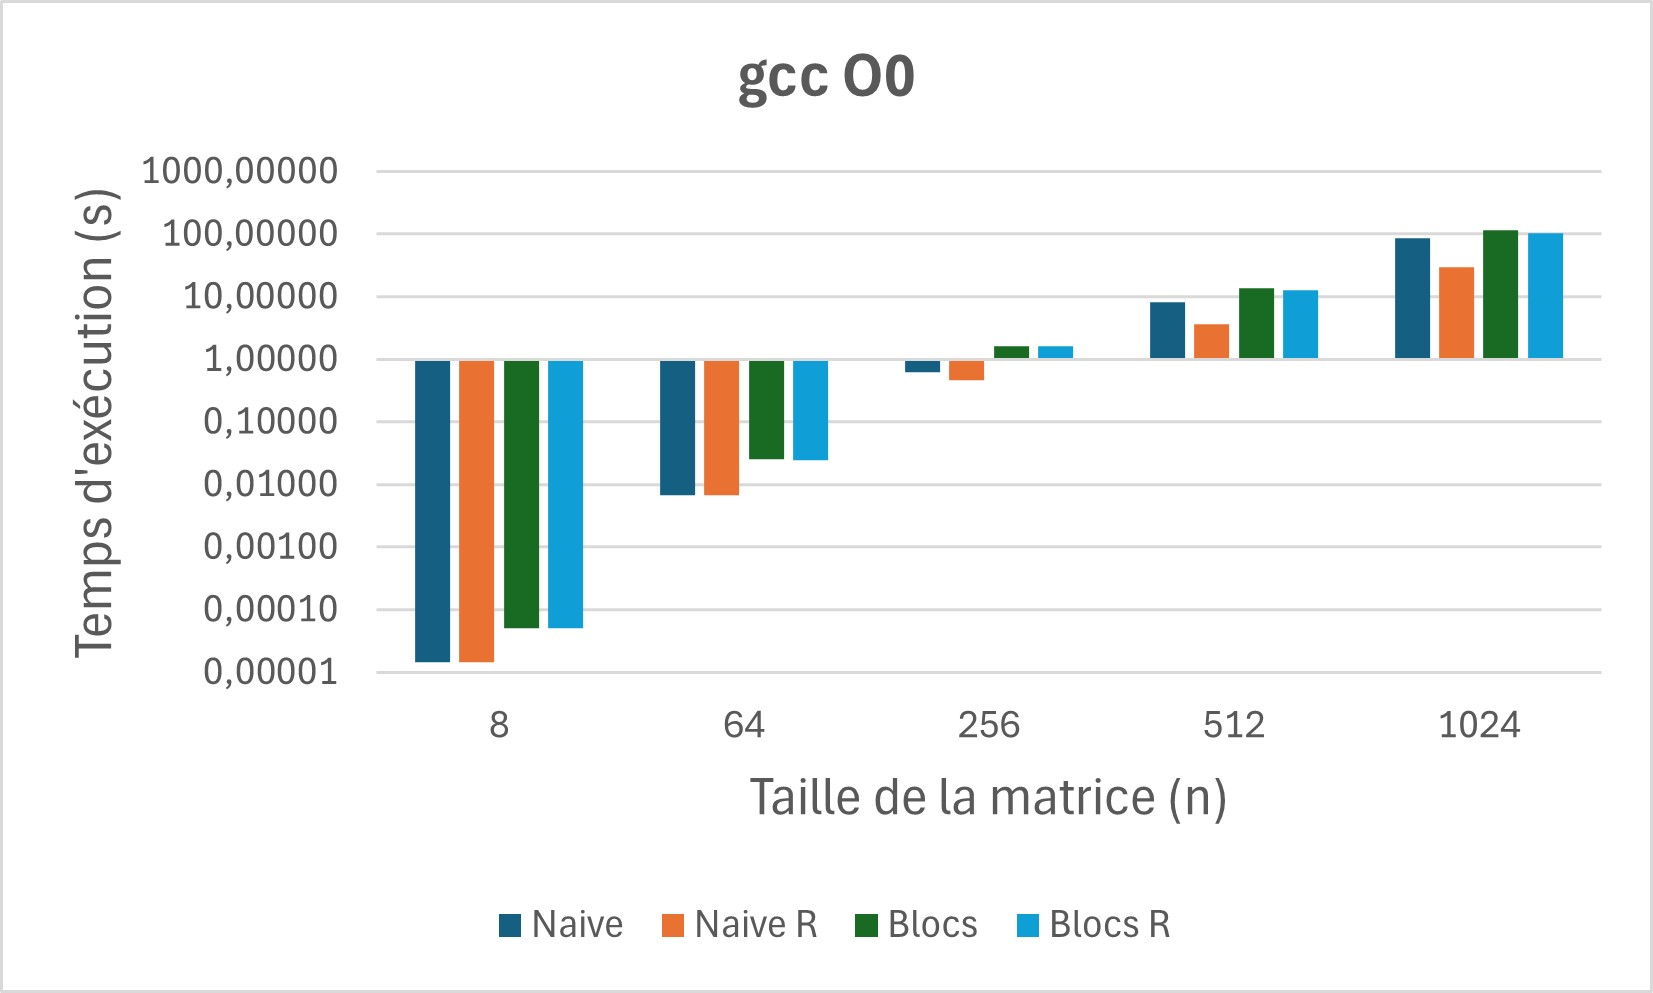
\includegraphics[width=1\columnwidth]{Images/Temps_gcc0_ARM9.jpg}
    \caption{Temps d'exécution de l'algorithme avec optimisation gcc O0.}
    \label{fig:7}
\end{figure}

\subsubsection{gcc O1}

Vous trouverez ci-dessous les résultats de Speed Up utilisant l'optimisation gcc O1, comparés aux résultats obtenus avec gcc O0.

\begin{figure}[H]
    \centering
    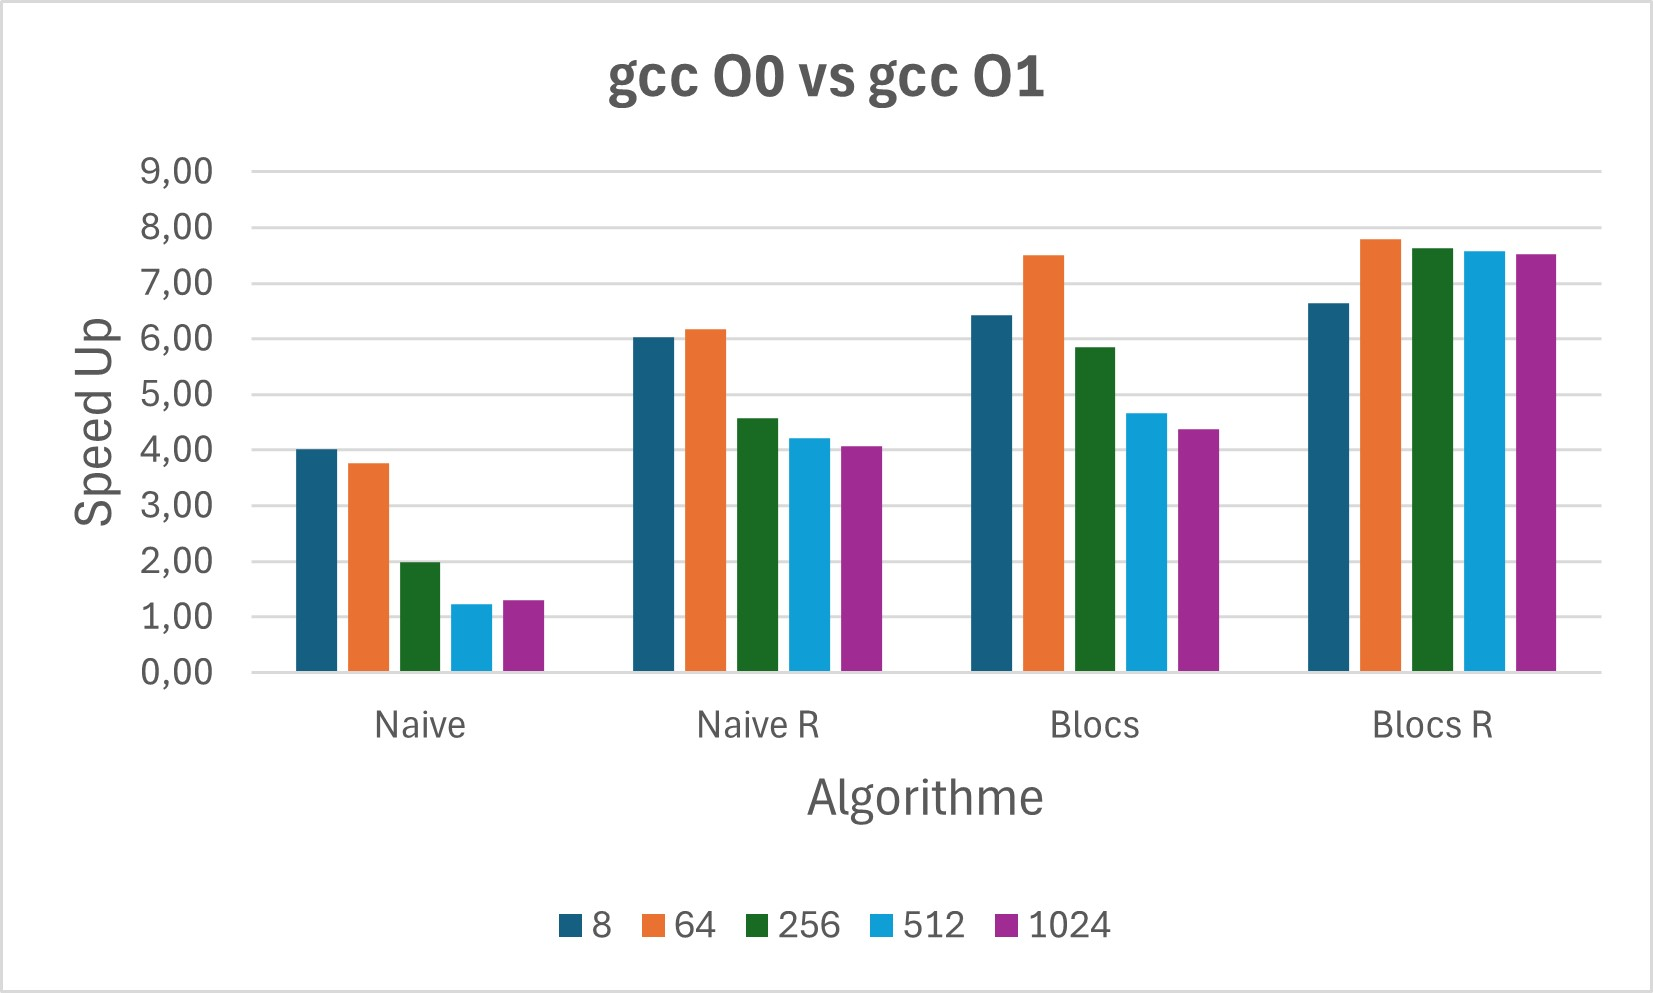
\includegraphics[width=1\columnwidth]{Images/SpeedUp1_gcc0vsgcc1_ARM9.jpg}
    \caption{Speed Up de l'optimisation de gcc O1 par rapport à gcc O0.}
    \label{fig:7}
\end{figure}

L'augmentation des performances entre gcc O0 et O1 est notable dans tous les algorithmes, en particulier dans les versions réorganisées et en bloc, avec des améliorations atteignant jusqu'à 7,79x sur des matrices de taille 64x64. Sur ARM9, l'amélioration est fortement influencée par l'optimisation des accès mémoire, puisque les versions blocs profitent mieux de la hiérarchie du cache et réduisent le nombre d'accès mémoire inutiles. Les algorithmes naïves montrent une Speed Up plus faible, probablement parce que les optimisations dans O1 (élimination du code redondant et simplification des boucles) sont moins efficaces dans les structures de boucles imbriquées qui ne donnent pas la priorité à la localisation des données.

\subsubsection{gcc O2}

Dans la figure suivante, vous pouvez voir les résultats Speed Up pour chacun des algorithmes utilisant l'optimisation gcc O2.

\begin{figure}[H]
    \centering
    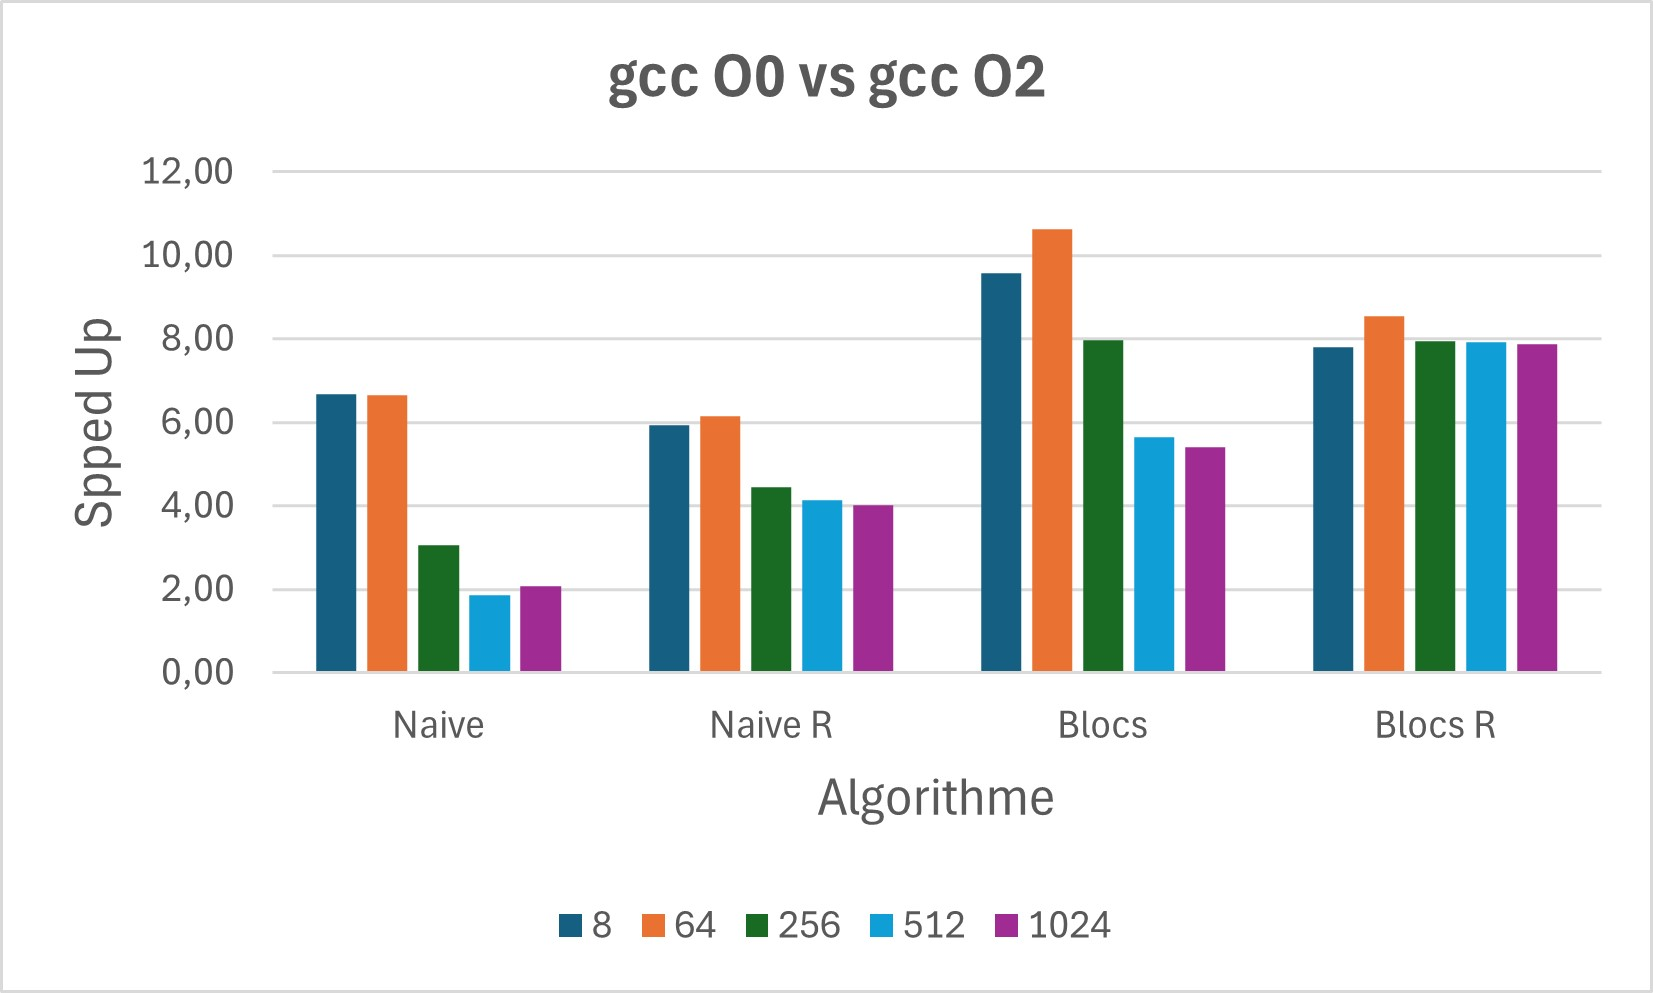
\includegraphics[width=1\columnwidth]{Images/SpeedUp1_gcc0vsgcc2_ARM9.jpg}
    \caption{Speed Up de l'optimisation de gcc O2 par rapport à gcc O0.}
    \label{fig:7}
\end{figure}


Les optimisations gcc O2 montrent une nouvelle amélioration des algorithmes de multiplication de blocs, atteignant jusqu'à 10,64x sur les matrices moyennes (64x64), indiquant que les optimisations O2 agressives (telles que la vectorisation et la désynchronisation des boucles) profitent aux algorithmes qui optimisent les accès à la mémoire. Sur ARM9, cela est crucial en raison de la puissance de traitement inférieure à celle d'un PC, ce qui rend l'efficacité de l'utilisation du cache et de la mémoire vitale. Les algorithmes naïves ont une amélioration plus limitée, car la structure de la boucle n'est pas aussi propice aux optimisations de l'accès mémoire.


\subsubsection{gcc O3}

La figure suivante montre comment l'optimisation gcc O3 affecte le comportement des algorithmes de multiplication matricielle.


\begin{figure}[H]
    \centering
    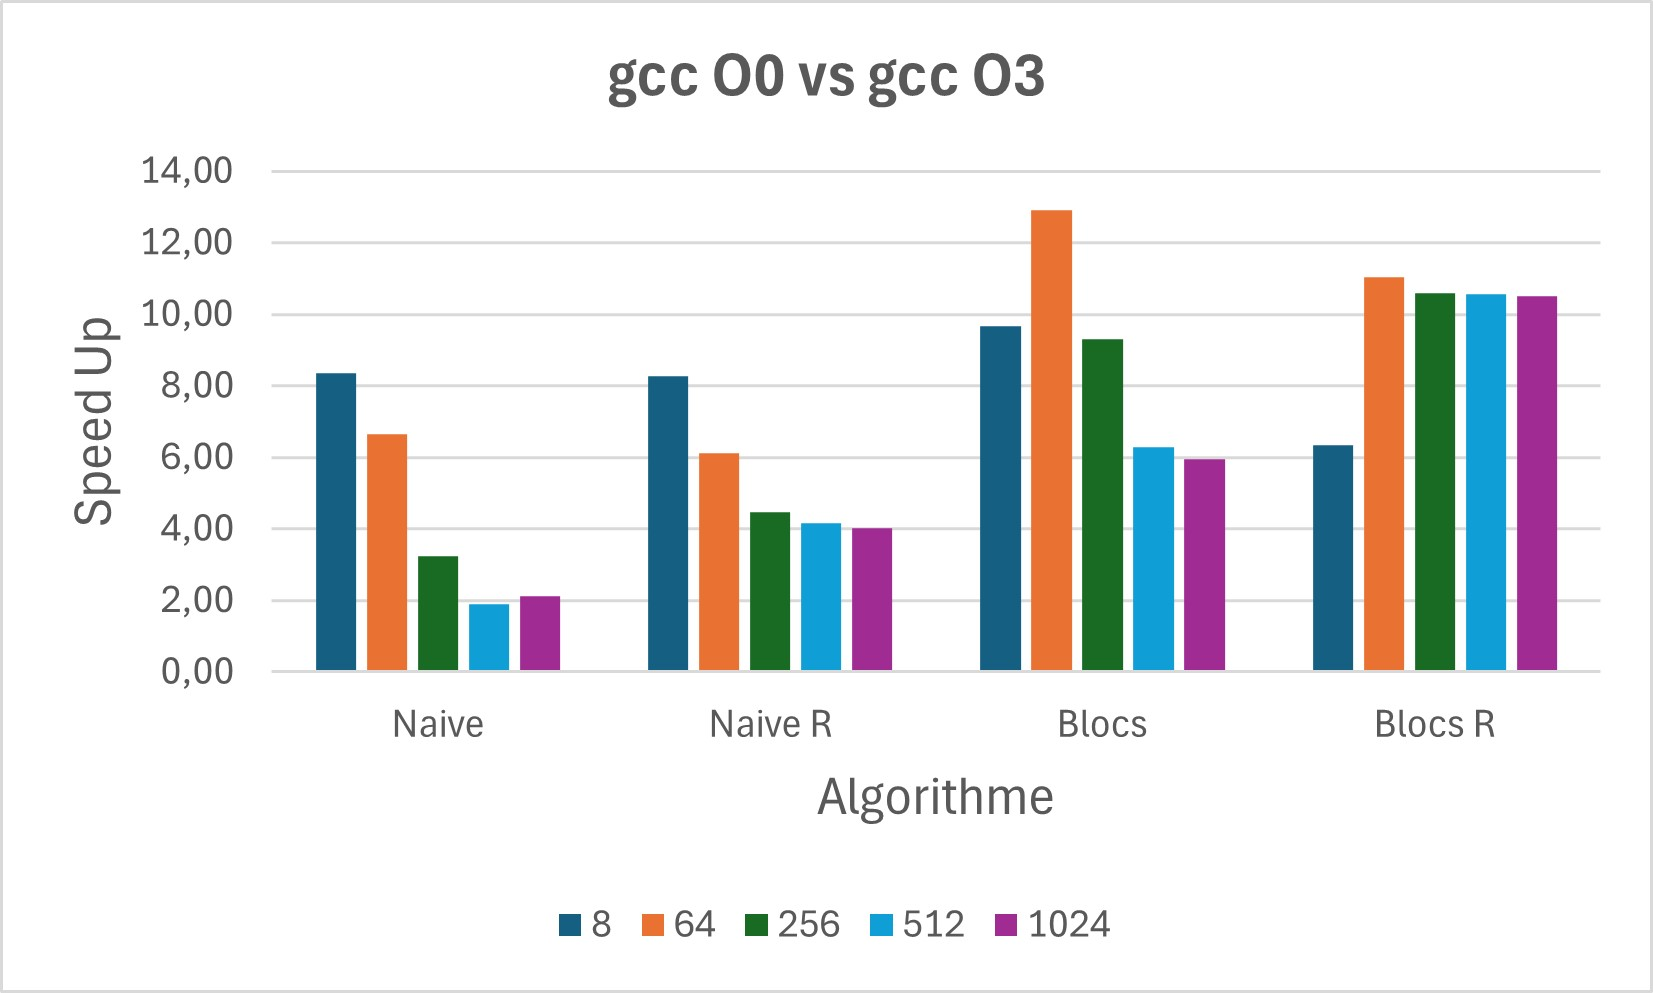
\includegraphics[width=1\columnwidth]{Images/SpeedUp1_gcc0vsgcc3_ARM9.jpg}
    \caption{Speed Up de l'optimisation de gcc O3 par rapport à gcc O0.}
    \label{fig:7}
\end{figure}

Gcc O3 obtient les meilleurs résultats sur les matrices moyennes (64x64), notamment dans les versions blocs, avec une Speed Up allant jusqu'à 12,91x. Cela indique que les optimisations avancées d'O3 (déroulement de boucles et inlining) profitent particulièrement aux implémentations qui font un meilleur usage du cache et minimisent les accès à la mémoire. Sur ARM9, où la mémoire constitue un goulot d'étranglement plus important que sur un PC, ces optimisations sont particulièrement efficaces dans les algorithmes qui réduisent l'accès aux données clairsemées. Cependant, les petites matrices n'en bénéficient pas autant, car les frais généraux liés à la gestion des optimisations dépassent les améliorations apportées à ces dimensions.

\subsection{Parallélisation par décomposition de tâche}

Nous cherchons à paralléliser la multiplication de matrices sur deux processeurs ARM en utilisant une BRAM partagée (mémoire vive bloc) pour améliorer les performances en répartissant la charge de calcul. 

La multiplication de matrices est une tâche intensive, et en utilisant deux processeurs, nous pouvons diviser le travail et réaliser la multiplication de manière plus efficace. Les scripts synchronisent les processeurs grâce à des sémaphores, ce qui leur permet de travailler simultanément sur différentes parties de la matrice. 

Ci-dessous, nous allons expliquer étape par étape le fonctionnement de ce processus, en détaillant comment les données sont partagées, comment la synchronisation est maintenue et comment la multiplication de matrices est effectuée.
\\
\subsubsection{Initialisation et configuration des matrices (ARM0)}
\begin{itemize}
\item \textbf{Ce qu’on fait} : ARM0 initialise les matrices A et B avec des valeurs aléatoires. La matrice de résultat C est initialisée à zéro.

\item \textbf{Pourquoi} : Ces matrices représentent les données à multiplier. ARM0 est responsable de leur création et de leur stockage dans la mémoire partagée (BRAM), afin que les deux processeurs y accèdent.

\item \textbf{Comment} : Les matrices sont de taille ajustable. ARM0 remplit A et B avec des valeurs aléatoires, et initialise C à zéro, car cette matrice contiendra les résultats de la multiplication.
\end{itemize}

\subsubsection{Configuration de la BRAM (mémoire partagée)}
\begin{itemize}
\item \textbf{Ce qu’on fait} : ARM0 configure la BRAM pour la rendre accessible par les deux processeurs. Cela permet à ARM0 et ARM1 d’accéder à la même mémoire.

\item \textbf{Pourquoi} : En utilisant une mémoire partagée, les deux processeurs peuvent lire et écrire les mêmes données sans les dupliquer, économisant ainsi de la mémoire et simplifiant la communication.

\item \textbf{Comment} : Le driver \texttt{XBram} est initialisé sur ARM0 et ARM1. ARM0 écrit les matrices A et B dans la BRAM pour qu'ARM1 puisse les lire et effectuer la multiplication.
\end{itemize}

\subsubsection{Sémaphores pour la synchronisation}
\begin{itemize}
\item \textbf{Ce qu’on fait} : ARM0 et ARM1 utilisent des sémaphores stockés dans la BRAM pour se synchroniser.

\item \textbf{Pourquoi} : Les deux processeurs travaillant en parallèle, il faut s'assurer qu'ils coordonnent correctement leurs actions. Par exemple, ARM1 doit attendre qu'ARM0 ait fini d'écrire les données avant de commencer à lire.

\item \textbf{Comment} : ARM0 écrit des drapeaux (ou indicateurs) spécifiques dans la BRAM, qui signalent à ARM1 quand commencer ou terminer certaines tâches. Par exemple :
\begin{itemize}
    \item \texttt{FLAG\_SEMAPHORE\_START\_READ} indique à ARM1 que les matrices A et B sont prêtes à être lues.
    \item \texttt{FLAG\_SEMAPHORE\_STOP\_MULT} indique que la multiplication est terminée.
\end{itemize}
\end{itemize}

\subsubsection{Lecture depuis la BRAM et multiplication (ARM1)}
\begin{itemize}
\item \textbf{Ce qu’on fait} : ARM1 attend le signal \texttt{FLAG\_SEMAPHORE\_START\_READ} d'ARM0. Une fois reçu, ARM1 lit les matrices A et B depuis la BRAM et commence à effectuer la multiplication pour sa partie.

\item \textbf{Pourquoi} : Cela garantit qu'ARM1 ne commence sa tâche qu'une fois les données prêtes, évitant ainsi des erreurs de concurrence.

\item \textbf{Comment} : ARM1 vérifie en continu le sémaphore. Dès qu'il détecte le signal, il lit les matrices et commence à multiplier.
\end{itemize}

\subsubsection{Multiplication en parallèle}
\begin{itemize}
\item \textbf{Ce qu’on fait} : ARM0 et ARM1 se partagent la multiplication de la matrice. ARM0 traite les lignes de 0 à 511 du script, tandis qu'ARM1 gère les lignes de 512 à 1023 du script.

\item \textbf{Pourquoi} : En divisant la tâche de manière parallèle, nous réduisons le temps total de calcul. Chaque processeur travaille sur une partie de la matrice, accélérant ainsi le processus.

\item \textbf{Comment} : Chaque processeur utilise un algorithme de multiplication de matrices pour sa section. ARM0 commence immédiatement après avoir écrit les données dans la BRAM, tandis qu'ARM1 attend le signal du sémaphore.
\end{itemize}

\subsubsection{Fin et mesure du temps (ARM0)}
\begin{itemize}
\item \textbf{Ce qu’on fait} : ARM0 mesure le temps nécessaire pour son calcul et attend qu'ARM1 ait terminé.

\item \textbf{Pourquoi} : Mesurer le temps nous permet d'évaluer l'amélioration des performances obtenue grâce à la parallélisation. ARM0 attend aussi ARM1 pour garantir que toute la multiplication est terminée avant de poursuivre.

\item \textbf{Comment} : ARM0 utilise \texttt{XScuTimer} pour mesurer le temps avant et après son calcul. Une fois sa partie terminée, il vérifie le sémaphore pour s'assurer qu'ARM1 a également fini.
\end{itemize}

\subsection{Explication des problèmes et analyse de performance}
\\
Au cours de l'exécution du code de multiplication de matrices sur la plateforme ARM, nous avons réussi à construire et à déboguer les deux projets d'application sans aucune erreur. Cependant, malgré l'exécution réussie, les résultats attendus n'étaient pas visibles dans la sortie de la console. Cette absence de sortie peut être attribuée à plusieurs facteurs, comme :
\\
\begin{itemize}
    \item \textbf{Problèmes de synchronisation} : Les indicateurs utilisés pour la synchronisation entre les deux processeurs (ARM0 et ARM1) peuvent ne pas avoir été gérés correctement. Si le timing de l'écriture ou de la lecture de chaque processeur à partir de la BRAM est désaligné, les résultats attendus peuvent ne pas être disponibles pour affichage lorsqu'ils sont demandés.

    \item \textbf{Gestion de la mémoire} : Il est crucial de vider le cache et de s'assurer que les données dans la BRAM sont synchronisées avec les données dans les registres du CPU. Tout échec à maintenir cette synchronisation peut entraîner la lecture de données obsolètes ou non initialisées.

    \item \textbf{Sortie de console} : La méthode d'affichage des résultats dans la console peut ne pas avoir été correctement configurée ou exécutée. Si la console ne reçoit pas correctement les données, la sortie attendue ne s'affichera pas.

    \item \textbf{Erreurs logiques dans le code} : Bien que la construction ait réussi, des erreurs logiques dans l'implémentation de la multiplication de matrices pourraient potentiellement empêcher le calcul des résultats corrects. Cependant, cela semble moins probable compte tenu de la structure des algorithmes de multiplication.
\end{itemize}
\\
\subsection{Analyse de performance théorique}
\\
Pour obtenir un aperçu de la performance des algorithmes implémentés, nous avons réalisé une analyse théorique basée sur les temps d'exécution obtenus en compilant le code C à l'aide de GCC avec le drapeau d'optimisation \texttt{-O3}. Ce niveau d'optimisation est conçu pour améliorer les performances du code par divers moyens tels que le déroulement de boucles, l'inlining et d'autres optimisations avancées.
\\
Dans notre analyse, nous avons constaté que le temps d'exécution des algorithmes parallélisés mis en œuvre sur la plateforme ARM était d'environ la moitié du temps d'exécution observé avec la version non parallélisée compilée avec GCC \texttt{-O3}. Cette amélioration significative des performances peut être attribuée à plusieurs facteurs :
\\
\begin{itemize}
    \item \textbf{Exécution parallèle} : Le principal avantage de l'utilisation de plusieurs processeurs est la capacité à exécuter différentes parties du calcul simultanément. Cela réduit le temps d'exécution global par rapport à une approche mono-thread, où les opérations doivent être réalisées séquentiellement.

    \item \textbf{Multiplication en Blocs et Naïve} : Les algorithmes mis en œuvre (multiplication naïve et multiplication par blocs) sont optimisés pour une exécution parallèle. En divisant le travail en plus petits blocs et en permettant à chaque processeur de calculer son bloc assigné indépendamment, nous atteignons une meilleure utilisation des ressources computationnelles.

    \item \textbf{Utilisation de la bande passante mémoire} : L'utilisation de la BRAM pour stocker les matrices A, B et C permet des temps d'accès plus rapides par rapport à la mémoire externe. Cela peut réduire considérablement la latence associée aux transferts de données, améliorant ainsi les performances.

    \item \textbf{Efficacité algorithmique} : Les algorithmes utilisés pour la multiplication de matrices (en particulier la variante de multiplication par blocs) sont bien adaptés à l'utilisation du cache, ce qui entraîne moins de ratés de cache et de meilleures performances par rapport aux méthodes de multiplication naïve.
\end{itemize}
\\
Alors, bien que nous ayons rencontré des problèmes pour visualiser les résultats directement dans la sortie de la console, la construction et le débogage réussis des deux projets d'application confirment l'intégrité globale de notre code. L'analyse de performance théorique indique que la parallélisation des algorithmes de multiplication de matrices sur l'architecture ARM est avantageuse. Le temps d'exécution atteint sur ARM0 et ARM1 est d'environ la moitié de celui de la version non parallélisée compilée avec GCC \texttt{-O3}. Cela démontre l'efficacité de l'utilisation de plusieurs processeurs pour des tâches intensives en calcul comme la multiplication de matrices, ouvrant la voie à de futures optimisations et améliorations de notre mise en œuvre.

\begin{figure}[H]
    \centering
    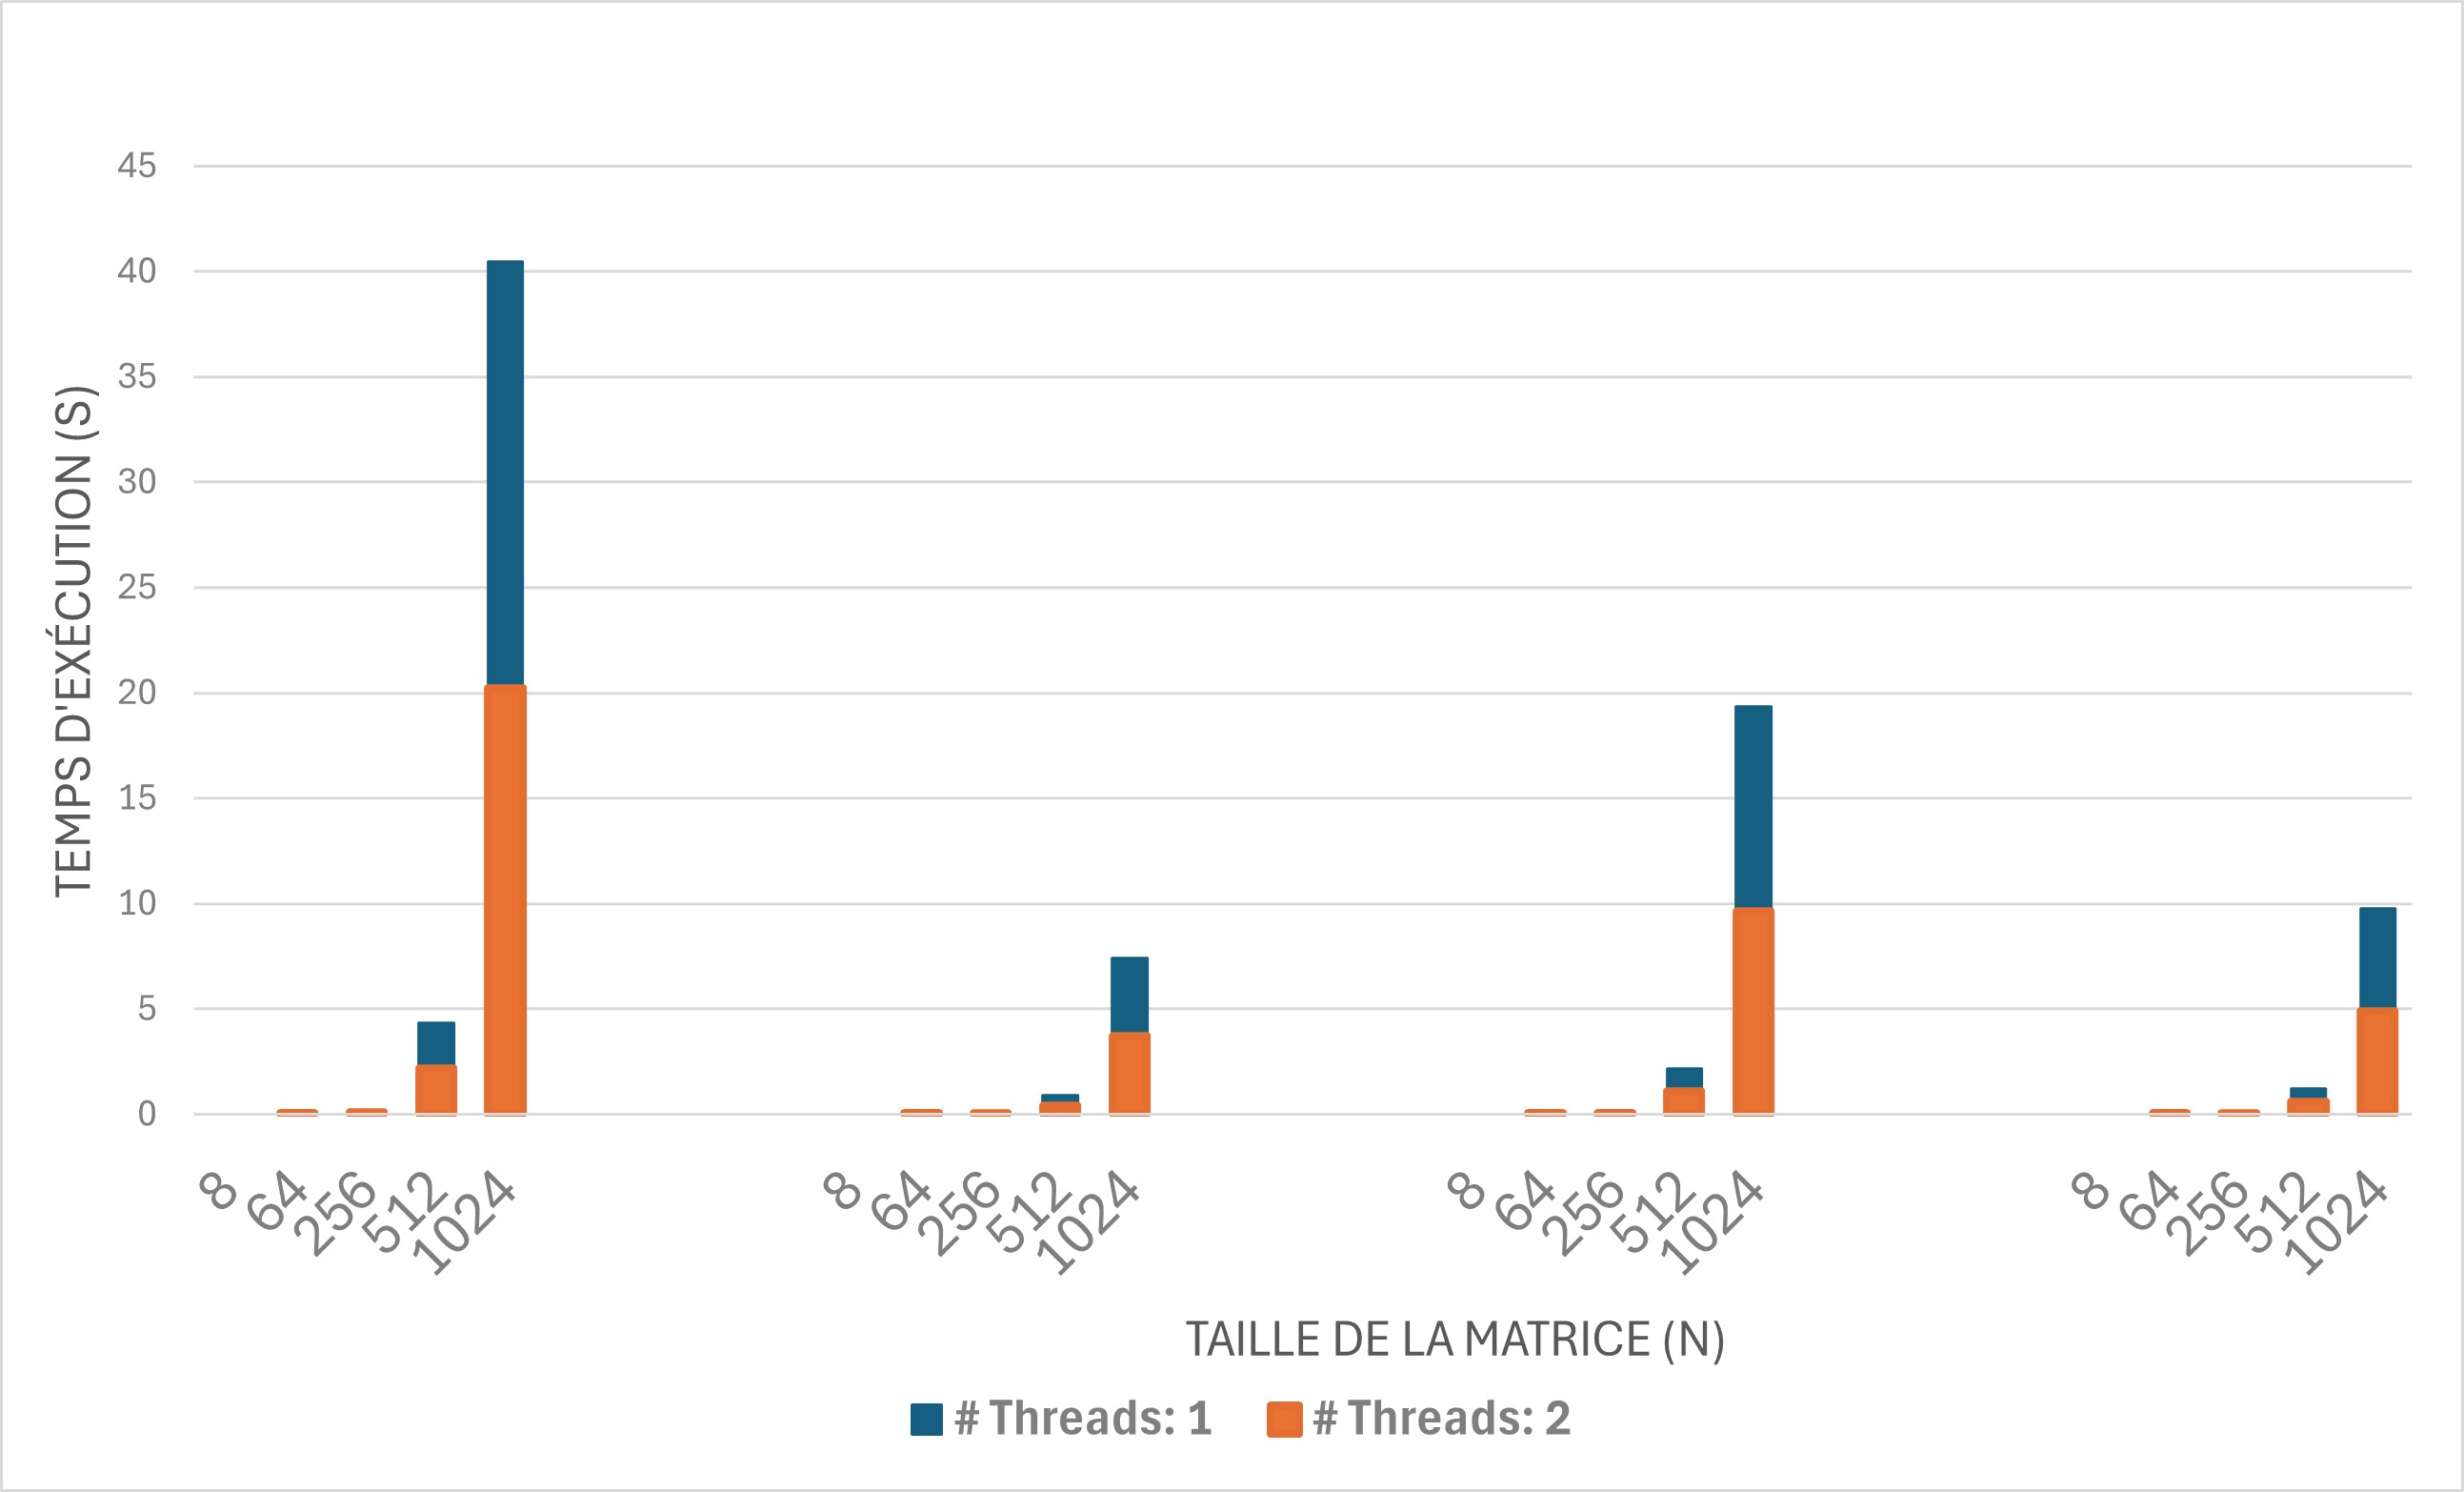
\includegraphics[width=1\columnwidth]{Images/ARM9_PARA.jpg}
    \caption{Comparaison des Temps d'Exécution : Mono-thread -o3 vs. Parallèle}
    \label{fig:7}
\end{figure}

\end{document}
